\documentclass[fleqn]{article}
\usepackage{brochure-venturis}
\def\wLaTeX{L\kern-.25em\raisebox{.5ex}{\fontsize{70}{0}\selectfont
    \textsc{a}}\kern-.12em T\kern-0.1667em\raisebox{-.5ex}{E}\kern-.1em X}
\begin{document}
\noindent\begin{tabular}{
  @{}%	                   flush left margin
  b{.35\columnwidth}%	   logo
  @{\hspace{.03\columnwidth}}%        gap
  >{\huge\centering\color{DarkBlue}}p{.62\columnwidth}%	   headline
  @{}%                     flush right margin
}
  \raisebox{-55pt}{%
    
\includegraphics[width=.37\columnwidth]{images/logo.jpeg}
    }
&
     University of Victoria\linebreak
     Horticulture Club\par\vspace{8pt}\hrule height3pt
  \fontsize{16}{18}\selectfont\itshape
  \par\bigskip
  May 2023 Newsletter\linebreak
\end{tabular}

\noindent\begin{tabular}{@{}
                         p{.38\columnwidth}%		blurb
		         @{\hspace{.04\columnwidth}}% 	gap
		         p{.58\columnwidth}%		quotes
		         @{}%			implicit margin
}

% Left Column
\sffamily\lite\fontsize{16}{18}\selectfont\raggedright 
Spring events that closed out the year: a plant sale and the Campus Community Garden Spring Social!
\par\bigskip

\small\rightskip=0pt
\subsection*{\sffamily Featured Plant: \emph{Heliamphora}}
\textit{Heliamphora} are a lesser-known—but no less remarkable—genus of highland carnivorous pitcher plant hailing on and around the Tepui mountains of Venezuela and small parts of Guyana and Brazil. The Tepuis are essentially floating islands (image below), with large plateaus situated above sheer cliff faces that can stand up to 1000 m tall. In fact, the tallest single-drop waterfall in the world, Angel Falls, is situated on one of the Tepuis. The ecosystems atop these plateaus have been largely isolated for millions of years, and as such different species of Heliamphora have evolved separately and are therefore found on specific mountains.
\par\bigskip
\includegraphics[width=.38\columnwidth]{images/tupey.jpg}
\emph{Above: Kukenán-tepui in Venezuela, taken by Paolo Costa}
\par\bigskip
Like all other carnivorous plants, Heliamphora have adapted carnivory as a means to acquire nutrients in a low-nutrient environment. The tops of the Tepuis are considered rain deserts and are extremely hostile to life. An abundance of rain paired with high wind speeds result in most nutrients being washed away off the mountain.
\quoted{(continued on Page 2)}
\par\bigskip
\vfill


% Upcoming Events Box, uncomment when have things to add
%\begingroup
%  \setlength{\fboxsep}{3pt}\noindent
%  \fbox{\vbox to8pc{\hsize=.38\columnwidth
%    \advance\hsize by-2\fboxsep\advance\hsize by-2\fboxrule
%    \null\vfill\normalsize\centering
%    Upcoming Events
%    \par\bigskip\footnotesize\tabcolsep1mm
%    \begin{itemize}[noitemsep]
%    \item Tomato Plant Sale: undetermined time/location.
%    \item More (Time / Location)
%    \item Upcoming (Time / Location)
%    \item Events (Time / Location)
%    \end{itemize}
%    \vfill}}
%\endgroup

&\large

% Right column
\lettrine[lines=3]{T}{he} past two months have been busy for the Horticulture Club, most notably with a plant sale that raised money for the club's operations next year. The plant sale was held in front of the Student Union Building on April 14th, where a variety of house plants and a few kinds of tomatoes were sold. All plants were originally purchased locally in Brentwood Bay. The event was a huge success and the executive team would like to extend appreciation to all of the members that helped fund the club through the purchase of a plant.
\linebreak\

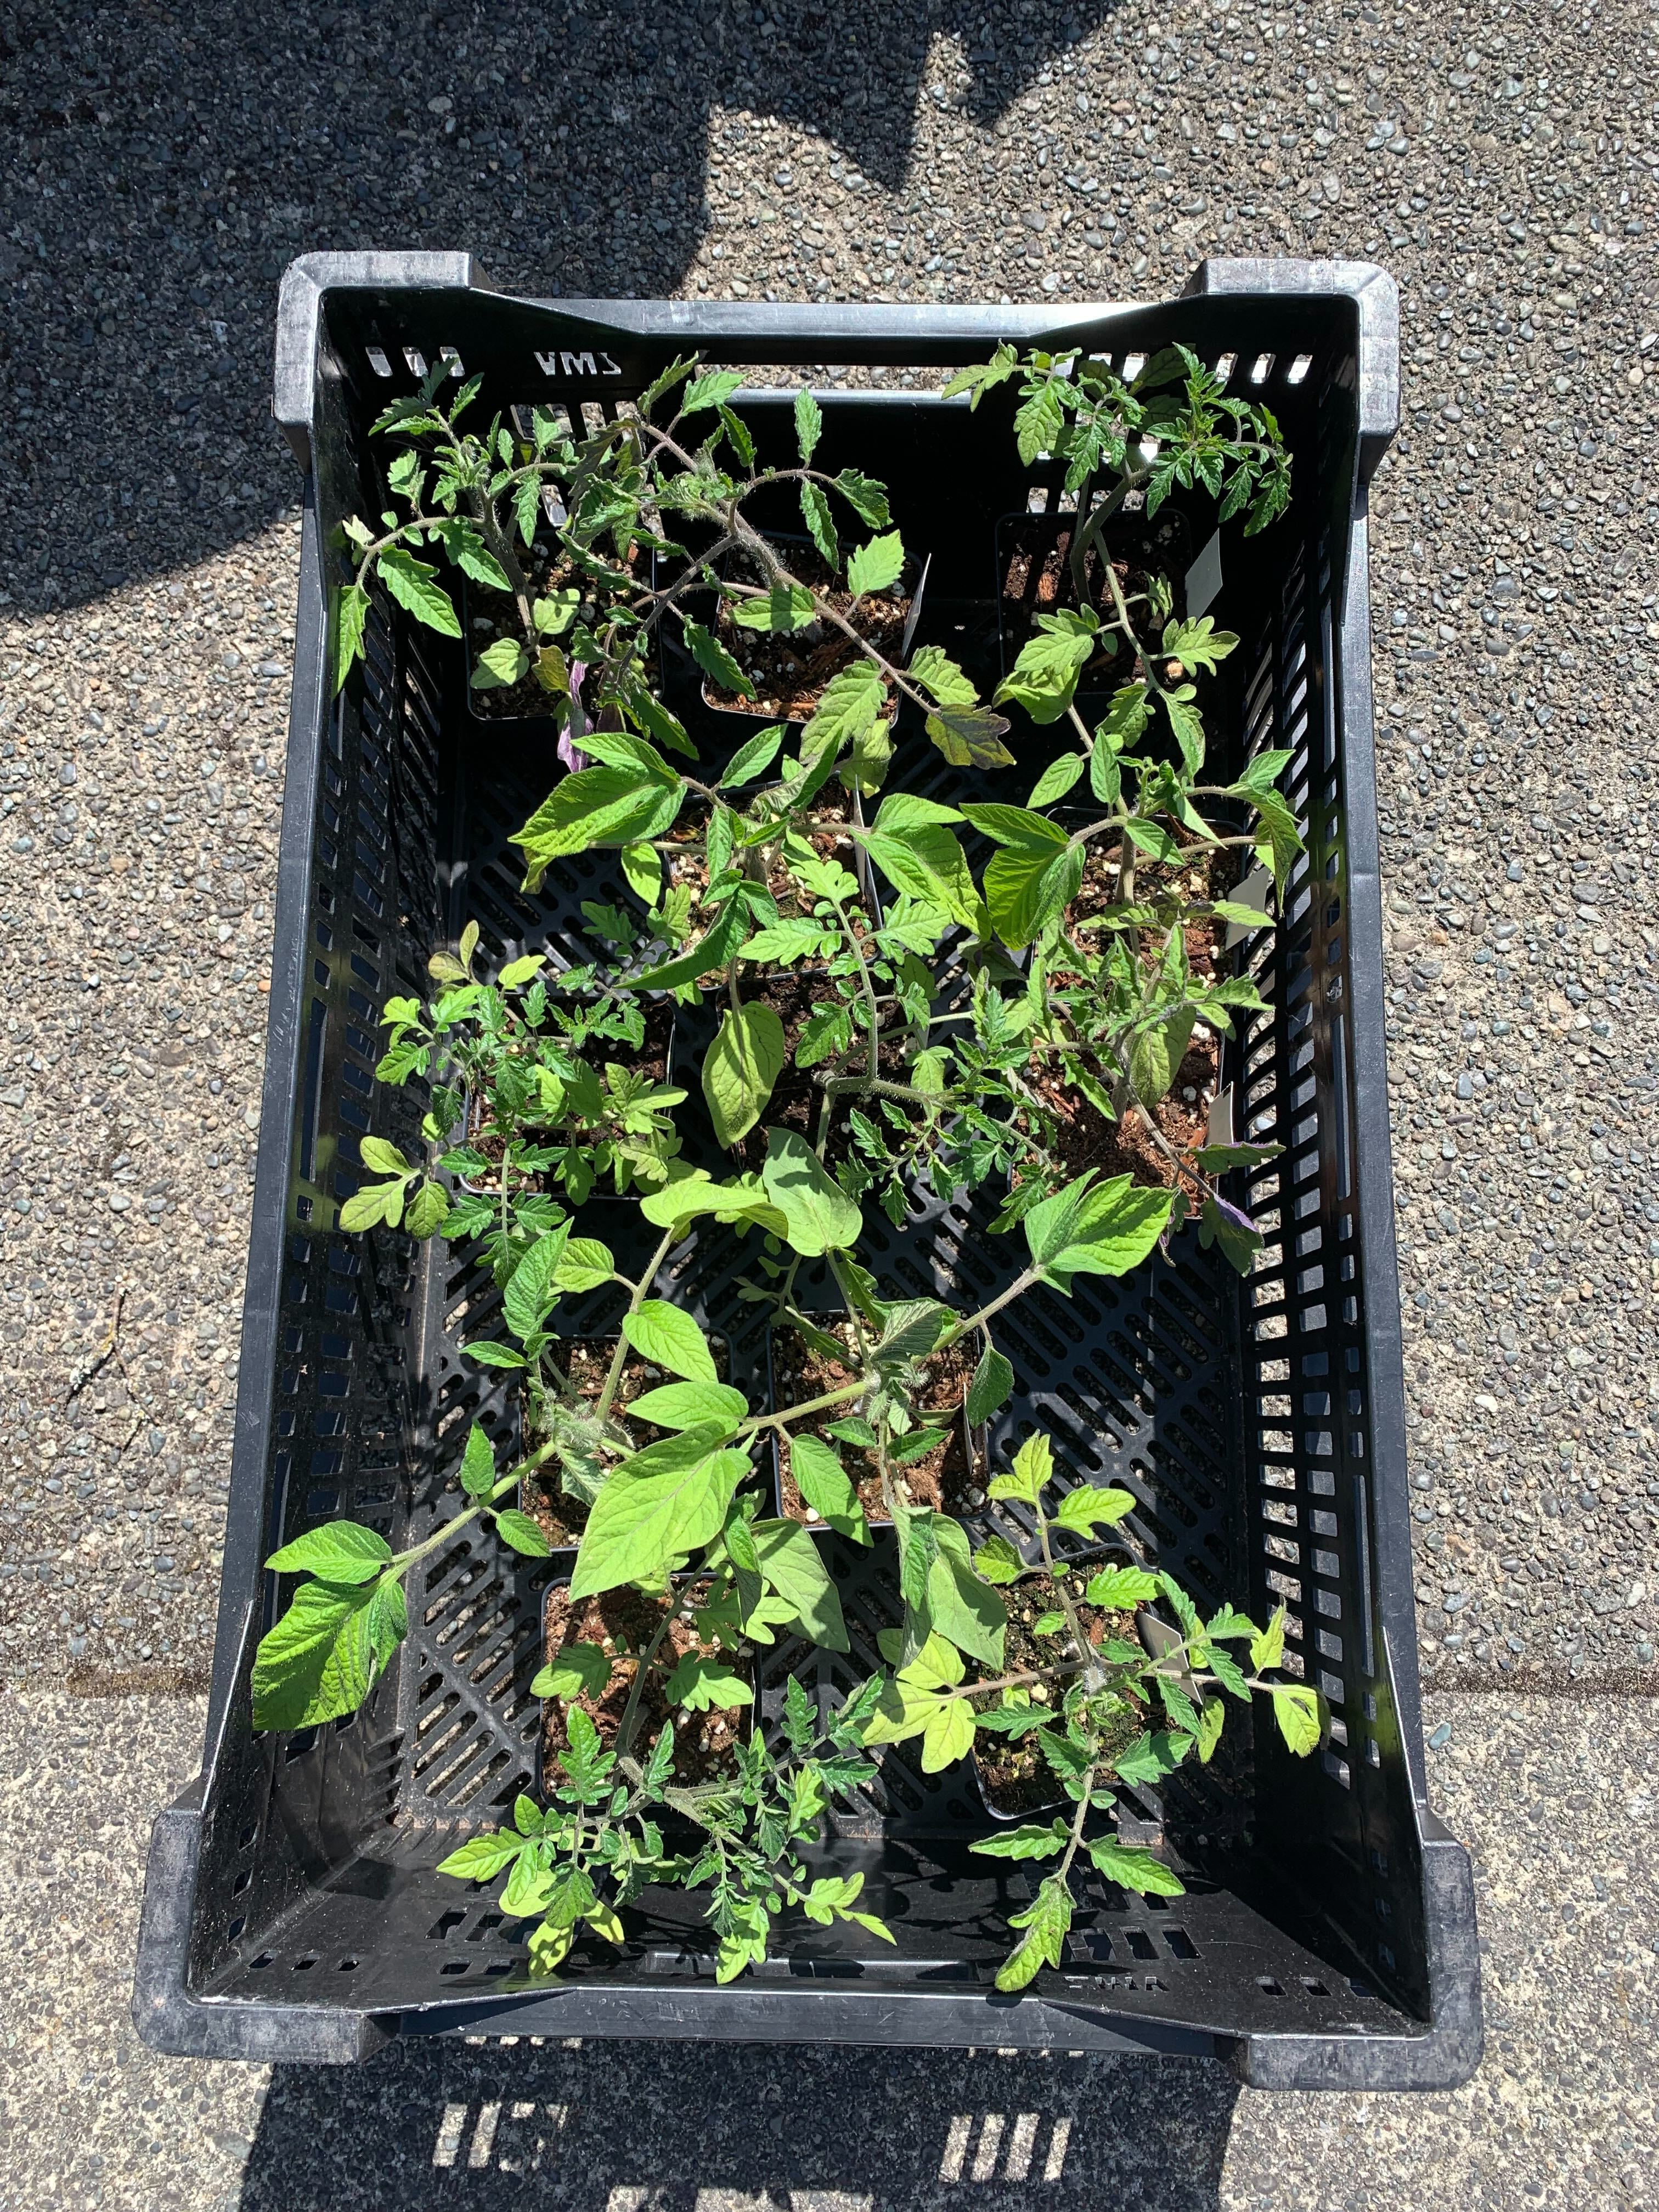
\includegraphics[width=.58\columnwidth]{images/plantsale.jpg}

\bigskip
\sffamily\lite\fontsize{10}{10}\selectfont\raggedright 
\emph{Above: A crate of plants sold at the Plant Sale this April.}
\sffamily\lite\fontsize{8}{8}\selectfont\raggedright 
\quoted{(continued on Page 2)}


\end{tabular}

\clearpage

%%%%%%%%%%%%%%%%%%%%%%%%%%%%%%%%%%%%%%%%%%%%%%%%%%%%%%%%%%%%%%%%%%%%%%%%
% Page 2

\noindent\begin{tabular}{@{}
                         p{.38\columnwidth}%		blurb
		         @{\hspace{.04\columnwidth}}% 	gap
		         p{.58\columnwidth}%		quotes
		         @{}%			implicit margin
}

% Left column
\sffamily\lite\fontsize{16}{18}\selectfont\raggedright 
\small\rightskip=0pt

\subsection*{\sffamily Featured Plant: \emph{Heliamphora} cont.}
The traps of Heliamphora are specialized leaves that attract, trap, and digest insects to gain essential nutrients. Nectar is produced by the “Nectar Spoon” of Heliamphora (in all described species apart from H. sarracenioides which instead has a number of nectar glands in the back of the trap): a variable appendage that is positioned on the upper-back of the pitcher in such a way that forces insects to walk across the inside of the pitcher to get to it. The pitcher is coated in a slippery wax, causing the insect to slip down into a pool of digestive fluids and eventually drown. To keep their pray from escaping, Heliamphora often have downward pointing hairs coating the inside of pitchers in addition to the wax that makes it near impossible to climb out, as well as a mechanism to limit the amount of fluid inside the pitcher such that prey cannot escape over the top of a filled pitcher.
There are 23 extant species of Heliamphora, all adapted to specific environments of the Tepuis, such as in massive, multiple-meter-in-diameter clusters or directly on cliff faces. Remarkably, as Heliamphora occur is such remote locations, there is little current threat of poaching, something that seriously affects many other genera of carnivorous plants, such as Nepenthes.
\quoted{Jack, Discord (11/23/2022)}
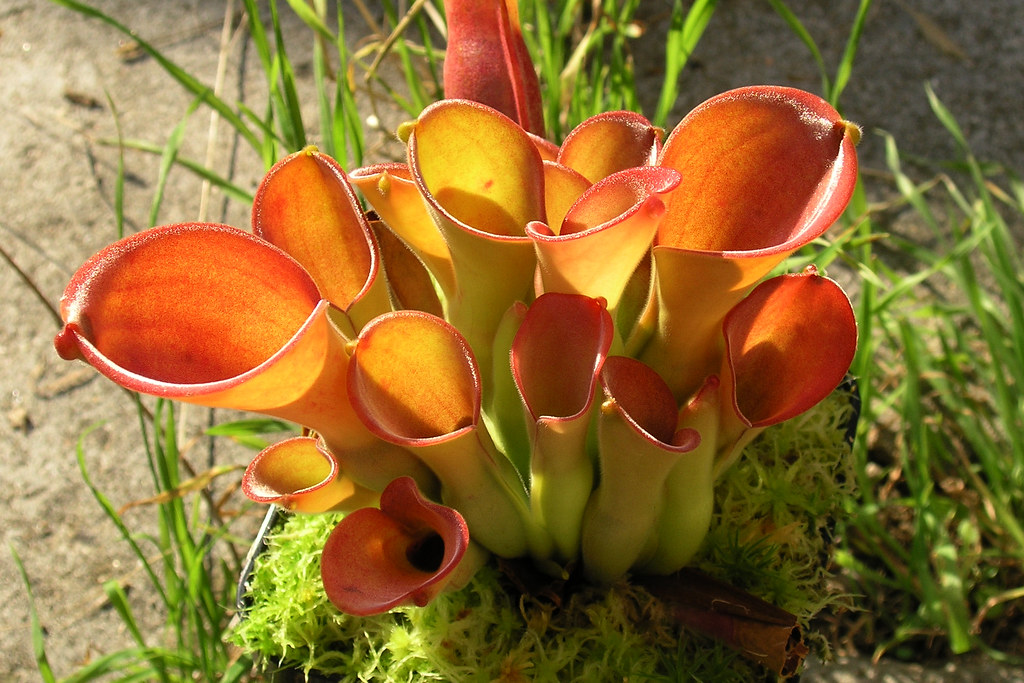
\includegraphics[width=.38\columnwidth]{images/heliamphora.jpg}
\emph{Above: \textit{Heliamphora exappendiculata} taken on Apacapa Tepui by Miloslav Dobšík}
\par\bigskip
\vfill

\begingroup
  \setlength{\fboxsep}{3pt}\noindent
  \fbox{\vbox to8pc{\hsize=.38\columnwidth
    \advance\hsize by-2\fboxsep\advance\hsize by-2\fboxrule
    \null\vfill\normalsize\centering
    Join the Club
    \par\bigskip\footnotesize\tabcolsep1mm
    Any events are free to attend for everyone, including non-members.
    If you would like to stay up to date with events, we recommend checking this newsletter or joining the club Discord, where you can chat with other members.
    If you would like to join the list of members, contact us on Instagram: @uvichorticulture
    \vfill}}
\endgroup

% Right column
&\large
\lettrine[lines=3] {}{Another} event many Horticulture Club members attended was the Spring Social, hosted by the Campus Community Garden on March 31st. Attendees enjoyed music, painting, an open mic and free food, all outside in the community garden. The weather got a little rainy but hot chocolate and tea came to the rescue. \linebreak\
\par\bigskip
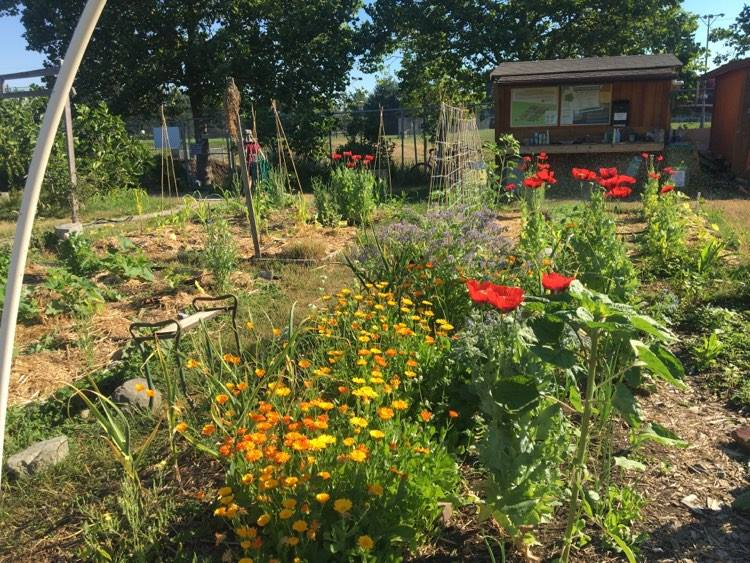
\includegraphics[width=.59\columnwidth]{images/communitygarden.jpeg}
\emph{Above: The community garden on a not-rainy day... a great spot for plant-themed events! Image by the UVic Campus Community Garden.}
\par\bigskip

\lettrine[lines=3] {}{Lastly}, a goodbye and a huge thanks from the executive team. Members' participation and enthusiasm, as well as recent purchases at the plant sale, all helped get this club off the ground! A number of non-graduating members will be resuming their positions next year, while some fresh undergraduates will step into executive roles. -- Thanks and see you this fall!
\par\bigskip
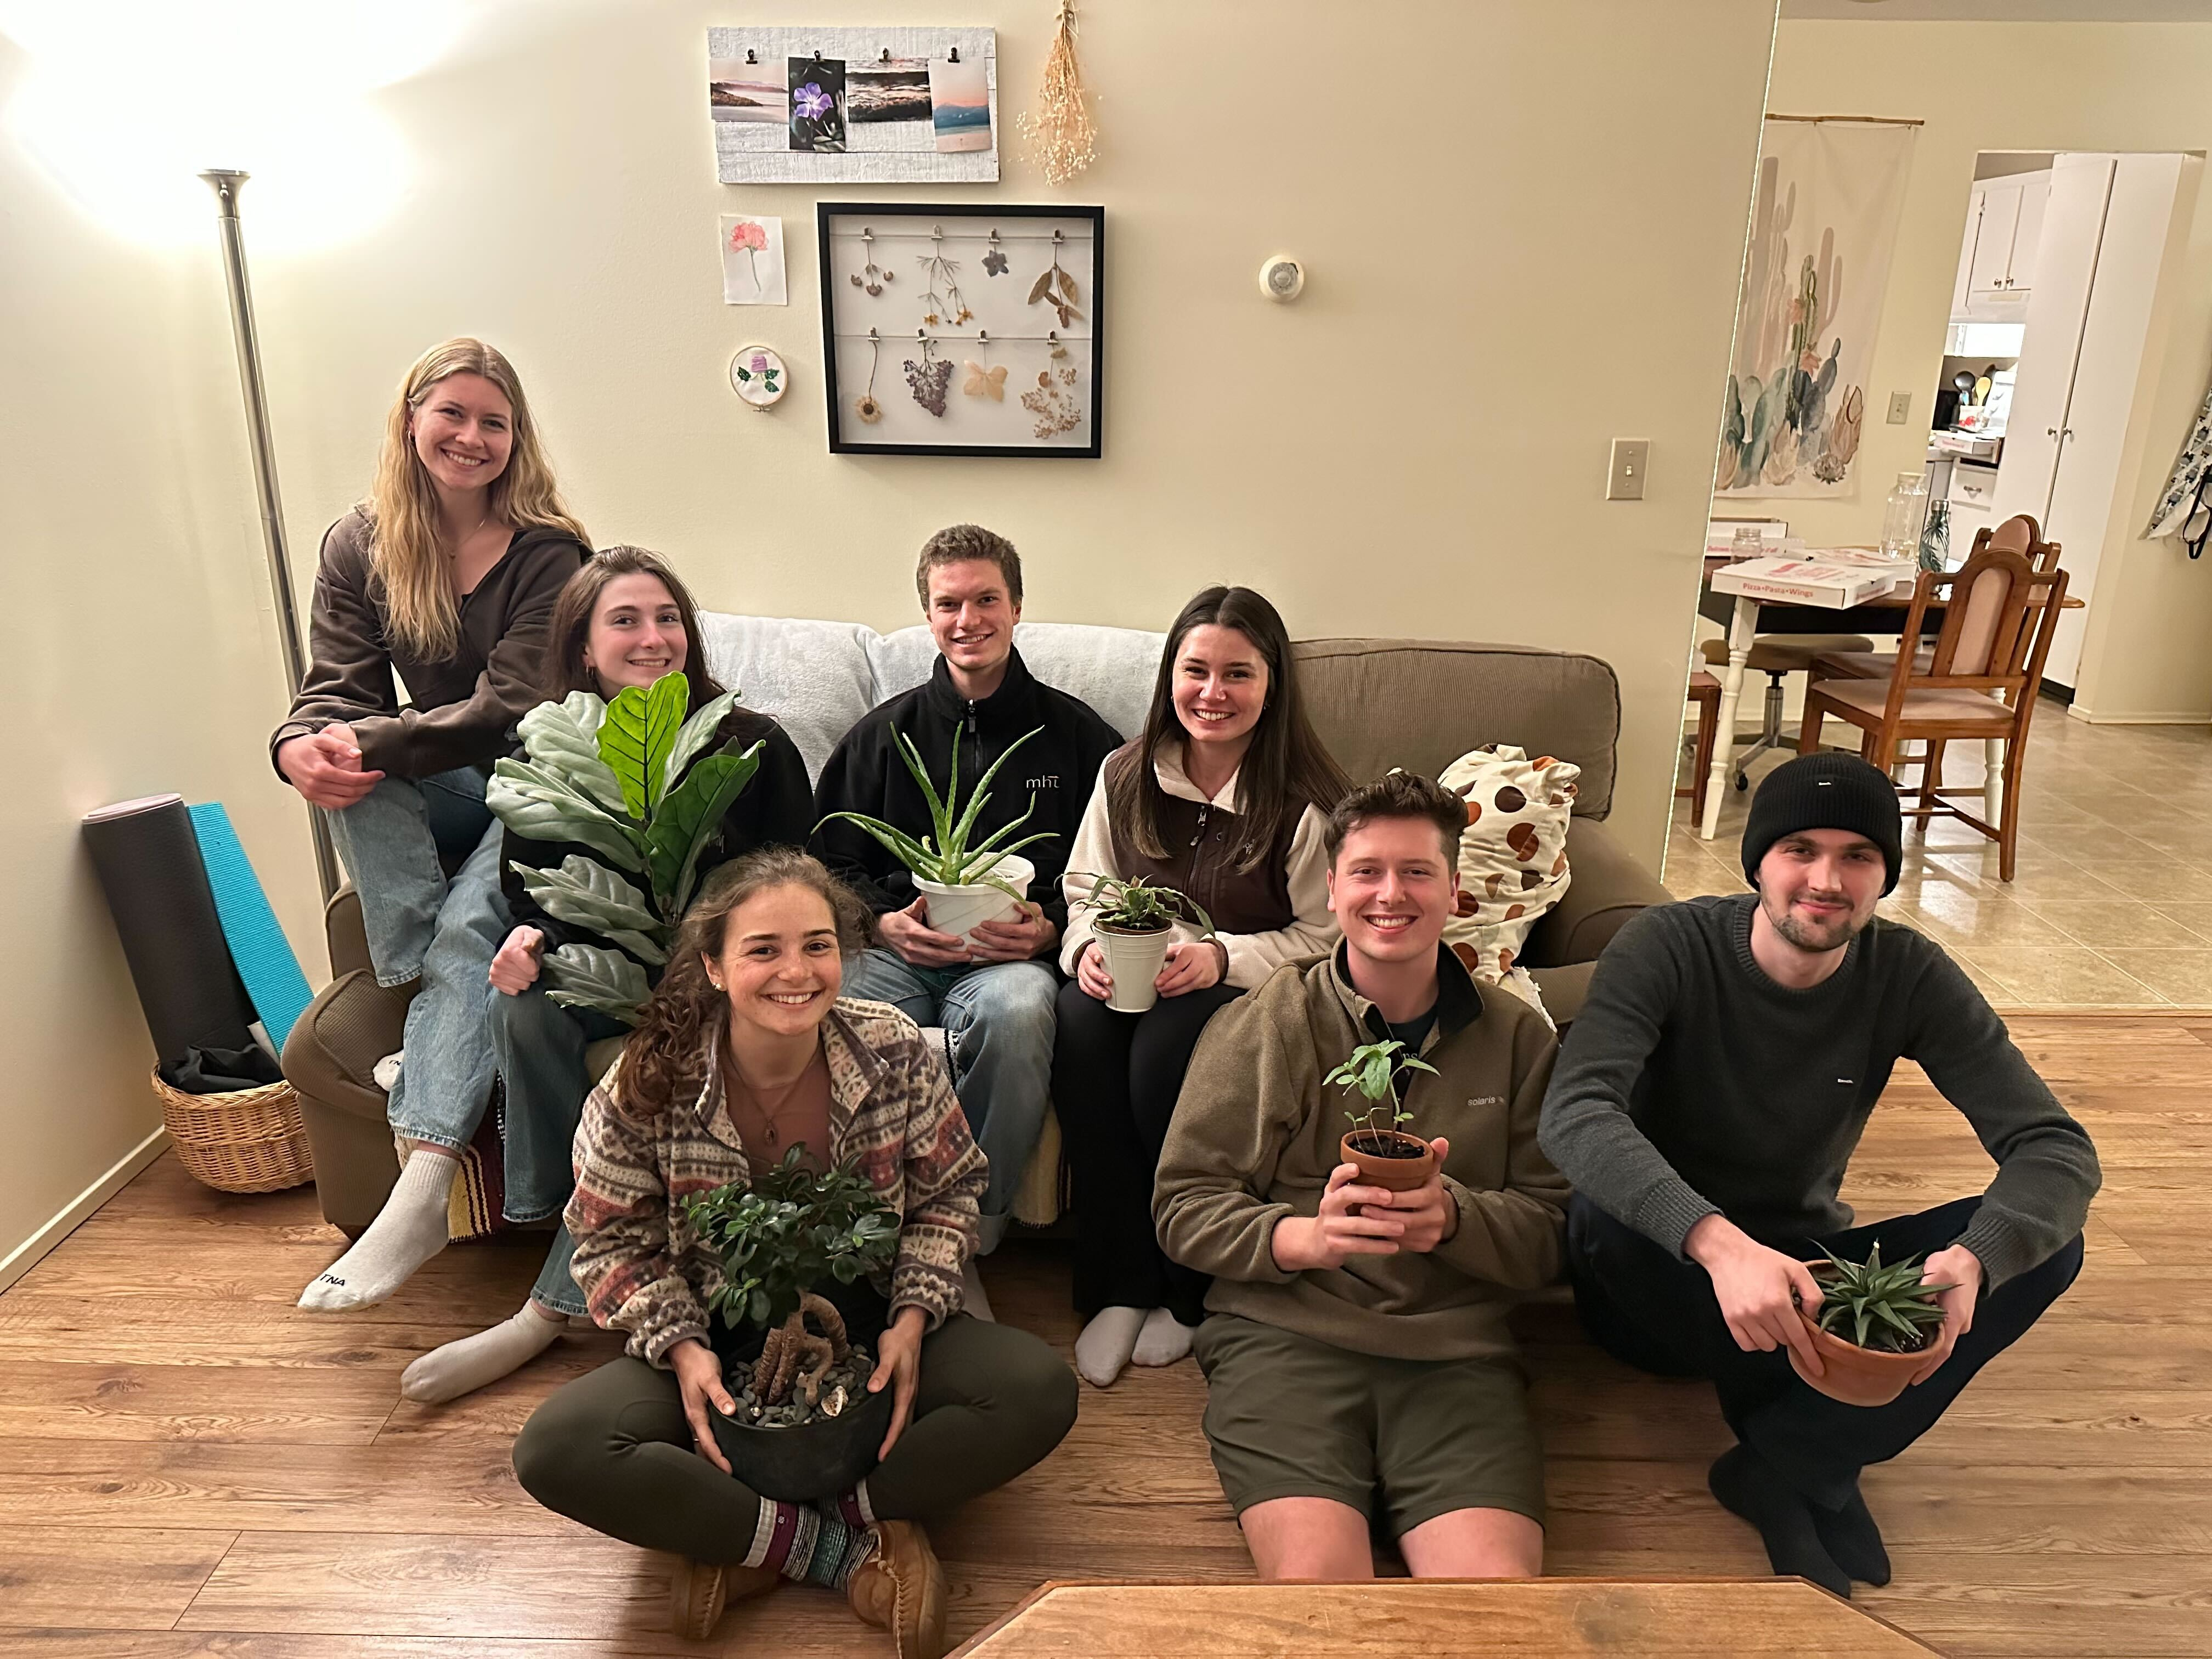
\includegraphics[width=.59\columnwidth]{images/team.jpg}
\par\bigskip
\emph{Above: A few members of this year's executive team. From left to right: Gracyn Kerfers, Catie Bass, Madeleine Guimond, Elliott Van der Wee, Zoe Koutsouropoulos, Keegan Thomas, Jack Smart. Photo by Simon Grieshaber-Otto.}





\vfill
\end{tabular}
\clearpage
\end{document}